\documentclass[12pt,a4paper]{article}
\usepackage[utf8]{inputenc}
\usepackage[T2A]{fontenc}
\usepackage[ukrainian]{babel}
\usepackage{fancyvrb}
\usepackage{pdflscape}

\usepackage{amsmath} % у преамбулі
\usepackage{array, multirow}
\usepackage{hyperref} % <-- Обов’язково підключіть цей пакет
\usepackage{caption}
\usepackage{booktabs}
\usepackage{subcaption} % для підписів (а), (б)
\usepackage{breqn} % Пакет для автоматичного перенесення виразів
\usepackage{mathtools} % Для додаткових можливостей, наприклад, для створення кастомних конструкцій

\usepackage{xcolor}

\renewcommand{\thetable}{№\arabic{table}}
\captionsetup[table]{name=Таблиця}  % замість "Табл." буде "Таблиця"

\usepackage{graphicx} % <-- Для роботи з \includegraphics
\usepackage{geometry}
\geometry{
    left=2cm,
    right=2cm,
    top=2cm,
    bottom=2cm
}

\begin{document}

    \begin{titlepage}

        \thispagestyle{empty}
        \begin{center}
        \large
        Національний технічний університет України\\
        «Київський політехнічний інститут імені Ігоря Сікорського»\\[1em]
        Факультет інформатики та обчислювальної техніки\\
        Кафедра загальної фізики
        \end{center}

        \vfill

        \begin{center}
        \textbf{\LARGE Фізика}\\[2em]
        \textbf{\Large Лабораторна робота №3-1}\\
        «Вивчення інтерференції світла. (Біпризма Френеля)» 
        \end{center}

        \vfill

        \begin{flushright}
        Виконав: студент 1 курсу ФІОТ, гр. ІО-41\\
        \textit{Давидчук А. М.}\\
        Залікова книжка № 4106\\[1em]
        Перевірив: \textit{Колган В.\,В.}
        \end{flushright}

        \vfill

        \begin{center}
        Київ -- 2025
        \end{center}

    \end{titlepage}

    \setlength{\parindent}{0pt}

    \textbf{\underline{Тема:}} «Вивчення інтерференції світла. (Біпризма Френеля)».

    \vspace{1em}

    \textbf{\underline{Мета:}} вивчення двопроменевий інтерференції світла за допомогою біпризми Френеля;
    визначення характеристик світлофільтра --- довжини хвилі в максимумі пропускання та ширини смуги пропускання.

    \vspace{1em}

    \textbf{\underline{Обладнання та прилади:}} установка для спостереження інтерференції.

    \vspace{1.5em}

    %%%%%%%%%%%%%%%%%%                      Теоритчні відомості                         %%%%%%%%%%%%%%%%%%%%%%%

    \begin{center}
        \textbf{\Large Теоретичні відомості}
    \end{center}

    \setlength{\parindent}{1.5em}

    Інтерференція є одним із проявів хвильових властивостей електромагнітного випромінювання,
    зокрема --- світла. Інтерференція полягає у характерному перерозподілі інтенсивностей у просторі при накладанні декількох
    хвиль за деяких умов. У даній роботі вивчається двопроменева інтерференція, при якій накладаються дві хвилі, і в кожній точці спостереження сходяться два промені.

    Сутність явища інтерференції найлегше зрозуміти на прикладі накладання двох ідеальних монохроматичних хвиль із однаковими частотами
    $\omega_1 = \omega_2 = \omega$ і напрямками коливань світлових векторів
    $\vec{E_1} \parallel \vec{E_2}$. Такі хвилі в заданій точці спостереження збуджують коливання, що задаються наступними рівняннями для проекцій світлових векторів:

    \begin{center}
        $E_1 = E_{01} \cos (\omega t - k_1 l_1 + \varphi_{01}) = E_{01} \cos (\omega t - \alpha_1)$,\\
        $E_2 = E_{02} \cos (\omega t - k_2 l_2 + \varphi_{02}) = E_{02} \cos (\omega t - \alpha_2)$.
    \end{center}

    де  $E_{01}$ і $E_{02}$ --- амплітуди, $l_1$ і $l_2$ --- шляхи, які
    проходять промені до точки спостереження, $k_1$ і $k_2$ --- хвильові числа, що визначаються до-
    вжиною хвиля як $k = 2\pi / \lambda$; $\varphi_{01}$ і $\varphi_{02}$ --- початкові фази хвиль, а
    $\alpha_1 = \varphi_{01} - k_1 l_1$ і $\alpha_2 = \varphi_{02} - k_2 l_2$ --- початкові фази коливань, які збуджуються
    хвилями в точці накладання.

    Результуючі коливання $E = E_1 = E_2$ найпростіше визначити за допомогою векторної діаграми (рис. 1),

    \begin{figure}[!ht]

        \renewcommand{\thefigure}{\arabic{figure}} % робимо "3.1", "3.2" і т.д.

        \centering
        % Підставляєте потрібний шлях та розмір зображення:
        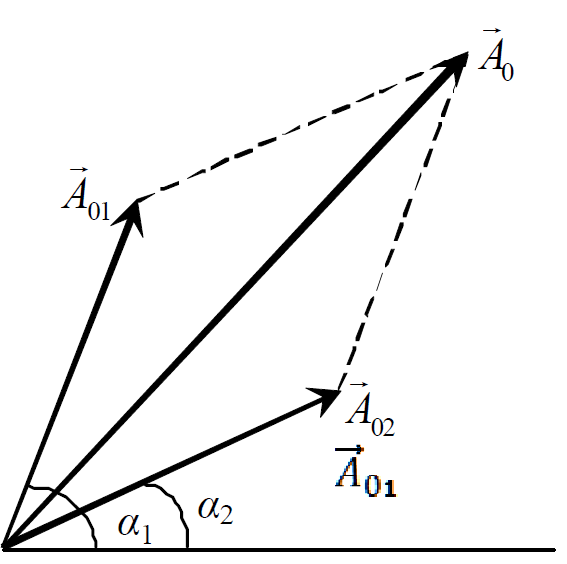
\includegraphics[width=0.35\textwidth]{1.png}
        % Підпис (зазвичай під малюнком):
        \caption{Векторна діаграма}
        % Мітка для посилань у тексті (\ref{fig:...})
        \label{fig1:schema}

    \end{figure}

    на якій коливання зображуються векторами $\vec{A}_{01}, \vec{A}_{02}$ з модулями  $A_{01} = E_{01}, A_{02} = E_{02}$, 
    які обертаються з кутовою швидкістю $\omega$ і напрямлені один до одного під
    кутом рівним різниці фаз цих коливань

    \begin{equation}
        \delta = \alpha_1 - \alpha_2 = (k_2 l_2 - k_1 l_1) - \delta_0
        \tag{1}
    \end{equation}

    де $\delta_0 = (\varphi_{02} - \varphi_{01})$ --- різниця початкових фаз даних хвиль.

    Відтак за теоремою косинусів можна записати:

    \begin{equation}
        E_0^2 = E_{01}^2 + E_{02}^2 + 2E_{01} E_{02} \cos \delta
        \tag{2}
    \end{equation}

    Інтенсивність світла визначається як середня величина густини потоку енергії і є прямо пропорційною квадрату амплітуди
    світлового вектора $I = \langle |S| \rangle \sim E_0^2$. Тому на основі виразу (2) можна записати:

    \begin{equation}
        I = I_1 = I_2 + 2\sqrt{I_1 I_2} \langle \cos \delta \rangle.
        \tag{3}
    \end{equation}

    Отже, при накладанні двох монохроматичних хвиль однакової частоти результуюча інтенсивність у точці
    спостереження не дорівнює сумі інтенсивностей кожної з хвиль окремо. В цьому й полягає сутність явища інтерференції.

    Такий ефект виникає через незалежність від часу різниці фаз хвиль і узгодженість коливань, які вони збуджують у точці спостереження.
    Такі хвилі називаються \textit{когерентними}. Отже, \textit{інтерференція спостерігається тільки при накладанні когерентних хвиль}.

    У випадку ідеальних монохроматичних хвиль однакової частоти, згідно з (1) $\cos \delta = const$, умова когерентності виконується точно. Але в реальних
    хвилях з ряду причин різниця фаз не є стабільною. Тому їхню інтерференцію
    можна бачити, лише коли за час спостереження\footnote{Час спостереження --- це мінімальний проміжок часу необхідний для реєстрації, приміром візуальної, розподілу інтенсивностей у просторі.}
    різниця фаз змінюється не дуже сильно так, що $\langle \cos \delta \rangle \neq 0$.

    \begin{center} \textbf{Різниця ходу променів. Умови максимумів і мінімумів} \end{center}

    З інтерференційної формули (3) випливає, що при $\cos \delta = 1$ утворюються максимуми інтенсивності
    
    \begin{center}
        $I_{max} = \left( \sqrt{I_1} + \sqrt{I_2} \right)^2$,
    \end{center}

    а при $\cos \delta = -1$ --- мінімуми інтенсивності

    \begin{center}
        $I_{min} = \left( \sqrt{I_1} - \sqrt{I_2} \right)^2$.
    \end{center}

    При цьому найбільша різниця інтенсивностей максимумів і мінімумів (контрастність), і найкращі умови спостереження інтерференції будуть при однакових інтенсивностях пучків
    $I_2 = I_1$, коли $I_{max} = 4I_0$, і $I_{min} = 0$.

    Різниці фаз, які відповідають максимумам і мінімумам, відповідно, дорівнюють:

    \begin{equation}
        \tag{4}
        \begin{aligned}
        \delta_{\text{max}} &= \pm 2m\pi \\
        \delta_{\text{min}} &= \pm (2m + 1)\pi
        \end{aligned}
        \qquad m = 0, 1, 2, \ldots
    \end{equation}

    Ці умови можна записати зручніше за допомогою співвідношення (1) за умови
    $\delta_0 = 0$, яка звичайно виконується на практиці:

    \begin{center}
        $\displaystyle \delta = k_2 l_2 - k_1 l_1 = 2\pi \left( \frac{l_2}{\lambda_2} - \frac{l_1}{\lambda_1} \right) = 
        \frac{2\pi}{\lambda_0} \left( n_2 l_2 - n_1 l_1 \right)$,
    \end{center}

    де $\lambda_0 = 2\pi c/\omega$ --- довжина світлової хвилі у вакуумі, а $n_1$ і $n_2$ --- показники заломлення середовищ, у яких поширюються промені.

    \newpage

    Величина $L = nl$ називається оптичною довжиною шляху, або оптичним ходом променя\footnote{Якщо промінь проходить
    декілька ділянок із довжинами $l_i$ і різними показником заломлення $n_i$, то оптичний хід $L = \sum n_i l_i$},
    а величина

    \begin{center}
        $\Delta = n_2 l_2 - n_1 l_1 = L_2 - L_1$
    \end{center}

    називається \textit{оптичною різницею ходу} променів.

    Якщо промені поширюються в одному середовищі з показником заломлення $n$, то

    \begin{center}
        $\Delta = n(l_2 - l_1)$,
    \end{center}

    де різниця відстаней $l_2 - l_1$ називається \textit{геометричною різницею ходу}.

    Таким чином, різниця фаз у загальному випадку та в однорідному середовищі,
    відповідно, визначається через різницю ходу променів формулою:

    \begin{equation}
        \Delta_{max} = \pm m \lambda_0
        \tag{6}
    \end{equation}

    і

    \begin{equation}
        \Delta_{min} = \pm \left( m + \frac{1}{2} \right) \lambda_0 = \pm \left( 2m + 1 \right) \frac{\lambda_0}{2},
        \tag{6а}
    \end{equation}

    де число $m = 0, 1, 2, ...$ називається \textit{порядком} інтерференційного максимуму або мінімуму.

    \begin{center} \textbf{Інтерференційна картина при двопроменевій інтерференції} \end{center}

    \textit{\underline{Ширина смуги}} при переміщенні точки спостереження в певному напрямі різниця ходу променів періодично проходить через значення,
    що задовольняють умови (6) і (6а). Тому в області накладання когерентних хвиль утворюється багато інтерференційних максимумів і мінімумів.
    При цьому, як видно з формули (3), при переході від максимуму до мінімуму і навпаки інтенсивність плавно зменшується та збільшується.
    Тому на встановленому на шляху хвиль екрані спостерігається інтерференційна картина у вигляді впорядкованої системи світлих і темних смуг.
    Форма цих смуг залежить від геометрії хвильових поверхонь хвиль, які інтерферують, і розташування екрана.

    Як приклад розглянемо інтерференційну картину від двох розміщених 
    у повітрі на відстані $h$ одне від одного когерентних лінійних джерел
    $S_1$ і $S_2$ у вигляді довгих паралельних світних ниток перпендикулярних
    до площини рис. 2, які випромінюють світло з довжиною хвилі $\lambda$.
    Екран для спостереження розташовано паралельно до площини джерел на відстані $l$.

    \begin{figure}[!ht]

        \renewcommand{\thefigure}{\arabic{figure}} % робимо "3.1", "3.2" і т.д.

        \centering
        % Підставляєте потрібний шлях та розмір зображення:
        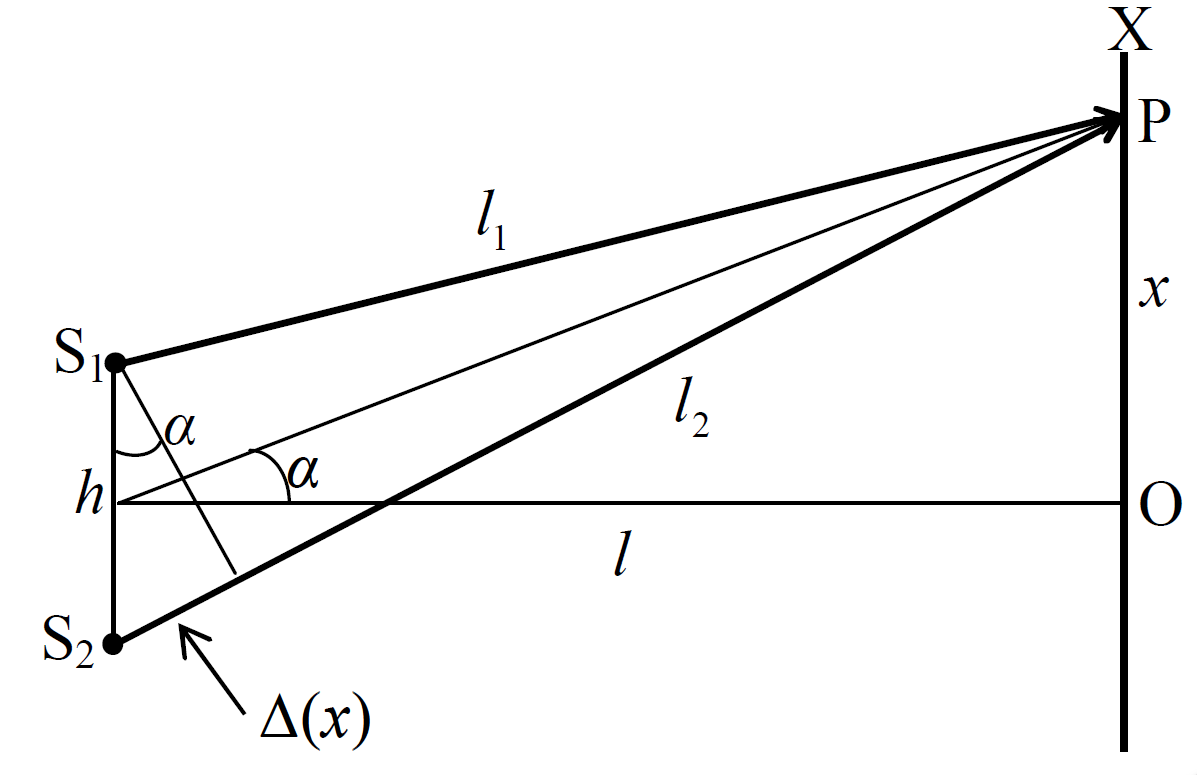
\includegraphics[width=0.35\textwidth]{2.png}
        % Підпис (зазвичай під малюнком):
        \caption{}
        % Мітка для посилань у тексті (\ref{fig:...})
        \label{fig2:schema}

    \end{figure}

    У випадку лінійних джерел інтерференційна картина на екрані має вигляд паралельних до
    $S_1$ і $S_2$ світлих і темних смуг, які утворюються згідно з
    умовами (6) і (6а). Для визначення їхнього розташування на екрані знайдемо залежність різниці ходу променів,
    які приходять у довільну точку $P$, від її координати $x$.
    У реальному досліді інтерференційні смуги можна спостерігати лише при малій відстані між джерелами
    $h << l$ і в малій центральній області екрана $x << l$. У такому разі кути
    $\alpha$ малі і за умови, що спостереження ведуться в повітрі ($n = 1$), можна записати:

    \begin{equation}
        \begin{aligned}
        \begin{array}{l}
        \Delta(x) = h\alpha \\
        x = l\alpha
        \end{array}
        \quad \Rightarrow \quad
        \Delta(x) = \frac{h}{l}x.
        \end{aligned}
        \tag{7}
    \end{equation}

    Підставивши цей вираз в умови (6) і (6а), отримуємо координати максимумів
    (світлих смуг) і мінімумів (темних смуг) на екрані:

    \begin{equation}
        x_{max} = \pm m \frac{\lambda l}{h},
        \tag{8}
    \end{equation}

    \begin{equation}
        x_{min} = \pm \left( m + \frac{1}{2} \right) \frac{\lambda l}{h}.
        \tag{8а}
    \end{equation}

    Із цих формул видно, що в точці О ($x = 0$) спостерігається центральна
    світла смуга порядку $m = 0$, а по обидва боки від неї --- симетрично розташовані світлі смуги порядків
    $m = 1, 2, ...$, розділені темними смугами (інтерференційними мінімумами).
    Крім того через малі розміри області спостереження відстані до джерел та інтенсивності смуг мають бути практично однаковими, як показано на рис. 3.

    \begin{figure}[!ht]

        \renewcommand{\thefigure}{\arabic{figure}} % робимо "3.1", "3.2" і т.д.

        \centering
        % Підставляєте потрібний шлях та розмір зображення:
        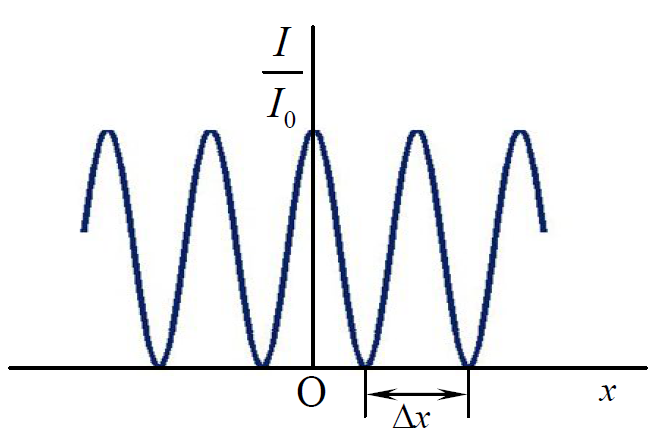
\includegraphics[width=0.35\textwidth]{3.png}
        % Підпис (зазвичай під малюнком):
        \caption{}
        % Мітка для посилань у тексті (\ref{fig:...})
        \label{fig3:schema}

    \end{figure}

    Лишається незмінною також ширина смуги $\Delta x = x_m - x_{m-1}$ (відстань між сусідніми мінімумами), для якої з виразу (8а) виходить:

    \begin{equation}
        \Delta x = \frac{\lambda l}{h}.
        \tag{9}
    \end{equation}

    Отже, інтерференційні смуги від двох лінійних джерел є еквідистантними,
    тобто розташованими на однаковій відстані одна від одної.

    \vspace{1em}

    \begin{center} \textbf{Інтерференційні схеми. Біпризма Френеля} \end{center}

    Описана вище інтерференційна картина (рис.3) утворюється при інтерференції двох ідеальних монохроматичних хвиль однієї частоти.
    Але дослід показує, що отримати такі строго когерентні хвилі і спостерігати інтерференцію світла від двох незалежних реальних
    джерел (за винятком лазерів) неможливо. Це зумовлено наявністю у реальних джерел лінійних розмірів і самим механізмом випромінювання
    тілами світла.

    Відомо, що тіла випромінюють світло не у вигляді неперервної хвилі, а
    як послідовність коротких імпульсів або обірваних «шматків» хвиль, які називають цугами.
    Ці цуги ніяк не пов’язані між собою і мають випадкові початкові фази.
    Тому початкова фаза в реальному світловому пучку дуже швидко
    й безладно змінюється. Так само змінюється і різниця фаз у пучках від незалежних джерел, тобто вони є некогерентними.
    Тому у формулі (3) $\langle \cos \delta \rangle = 0$
    і інтерференція відсутня. Але нестабільність початкових фаз можна подолати
    і спостерігати інтерференцію світла, скориставшись одним точковим монохроматичним джерелом.
    Якщо поділити його випромінювання на два пучки й спрямувати їх так, щоби промені проходили до точок спостереження різні
    шляхи, то початкові фази в обох променях кожної миті будуть однаковими, і
    різниця фаз (1) не буде залежати від часу.
    Тому поділені промені будуть когерентними і можна буде спостерігати інтерференцію.

    На практиці для отримання когерентних променів використовують різні способи поділу пучків, або
    \textit{інтерференційні схеми}.
    Одна з них --- схема з біпризмою Френеля --- використовується в даній лабораторній роботі.
    Біпризма Френеля має вигляд двох однакових призм із показником заломлення $n$
    і дуже малим заломлюючим кутом $\vartheta$, які з'єднані малими основами (рис. 4).

    \begin{figure}[!ht]

        \renewcommand{\thefigure}{\arabic{figure}} % робимо "3.1", "3.2" і т.д.

        \centering
        % Підставляєте потрібний шлях та розмір зображення:
        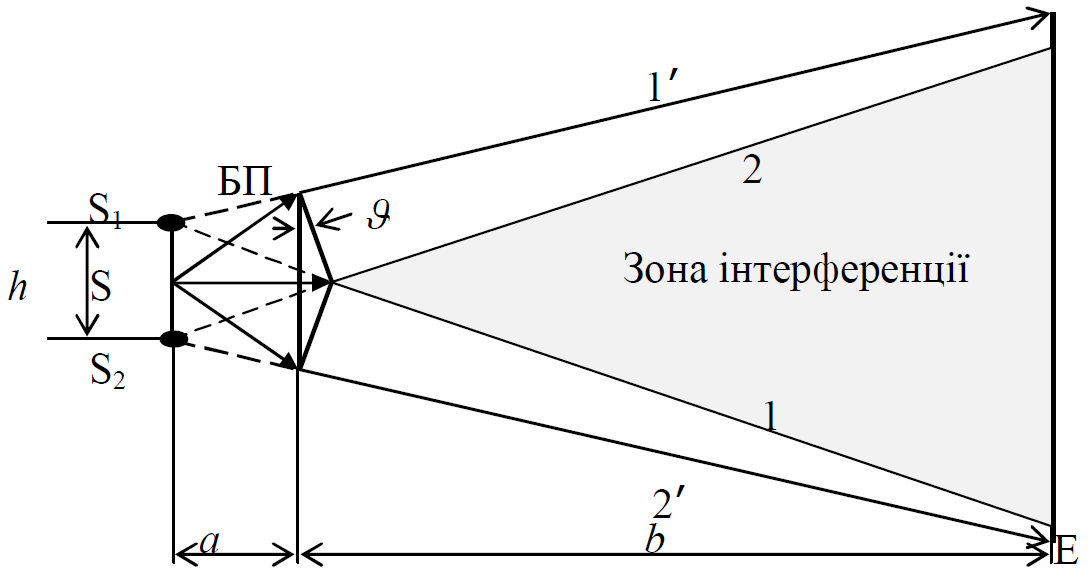
\includegraphics[width=0.5\textwidth]{4.png}
        % Підпис (зазвичай під малюнком):
        \caption{}
        % Мітка для посилань у тексті (\ref{fig:...})
        \label{fig4:schema}

    \end{figure}

    Як джерело використовується вузька щілина $S$, 
    що опромінюється монохроматичним світлом із довжиною хвилі $\lambda$ і
    розташована на деякій відстані $a$ від біпризми паралельно до ребра, як показано на рис. 4.
    Світло, що падає на біпризму, після заломлення в її половинах утворює два розбіжні пучки $1-1'$ і $2-2'$, які перекриваються в секторі 1-2 (\textit{зоні інтерференції}).
    Продовження заломлених променів перетинаються на лініях $S_1$ i $S_2$, які можна розглядати як уявні когерентні джерела світла, утворені поділом випромінюванням від одного дійсного джерела $S$.
    Тому в секторі перекривання пучків 1-2 відбувається двопроменева інтерференція, яку можна спостерігати у вигляді світлих і темних смуг на екрані $E$ розміщеному на деякій відстані $b$ від
    біпризми. Ширина смуги визначається формулою (9), в якій $l = a + b$, а відстань між когерентними джерелами визначається із закону заломлення і при
    малому заломлюючому куті біпризми $\vartheta$ дорівнює:

    \begin{equation}
        h = 2a(n-1)\vartheta.
        \tag{10}
    \end{equation}

    Отже, в досліді з біпризмою Френеля ширина інтерференційної смуги на екрані дорівнює

    \begin{equation}
        \Delta x = \frac{\lambda l}{h} = \frac{\lambda (a + b)}{2a(n-1)\vartheta}.
        \tag{11}
    \end{equation}

    У даній роботі, вимірюючи ширину інтерференційної смуги та відстань
    між уявними джерелами при заданій відстані від біпризми до екрана, можна
    визначити довжину хвилі в максимумі пропускання світлофільтра, який використовується в експерименті.

    \begin{center} \textbf{Інтерференційна картина від реальних джерел} \end{center}

    Окрім нестабільності початкових фаз є й інші несприятливі для спостереження інтерференції світла фактори, через що реальна
    інтерференційна картина суттєво відрізняється від показаної на рис. 3.
    Ці негативні фактори пов'язані з неповною монохроматичністю та лінійними розмірами реального джерела світла.

    Неповна монохроматичність світла має принциповий характер і випливає з того
    положення теорії, що всяка «обірвана» хвиля, зокрема цуг, визначається не однією
    частотою $\omega$ та довжиною хвилі $\lambda$, а певною \textit{спектральною шириною},
    тобто цілим інтервалом значень $\Delta \omega$ та $\Delta \lambda$.
    Через це у досліді з біпризмою чи в будь-якій іншій інтерференційній схемі різниця
    фаз поділених і формально когерентних променів завжди змінюються з часом.
    Отож вони можуть бути або тільки частково когерентними або взагалі
    некогерентними, якщо за час спостереження буде $\langle \cos \delta \rangle = 0$.

    Вплив неповної монохроматичності на інтерференцію в досліді з біпризмою
    проаналізуємо спочатку припустивши, що у спектрі випромінювання
    джерела $S$ присутні тільки дві довжини хвилі: $\lambda$ і $\lambda + \Delta \lambda$.
    Тоді розподіл інтенсивностей на екрані можна розглядати як суперпозицію двох
    інтерференційних картин, одна з яких створюється монохроматичними променями
    з довжиною хвилі $\lambda$ а інша --- з довжиною хвилі $\lambda + \Delta \lambda$.
    Ці картини характеризуються різною шириною смуги (формула (9)) і
    поступово «розповзаються», як показано на рис. 5а.

    \begin{figure}[h!]

        \centering
        \begin{subfigure}[b]{0.45\textwidth}
            \centering
            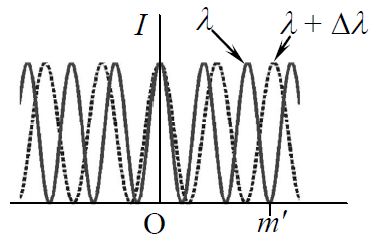
\includegraphics[width=\textwidth]{5a.png}
            \caption*{а)}
        \end{subfigure}
        \hfill
        \begin{subfigure}[b]{0.45\textwidth}
            \centering
            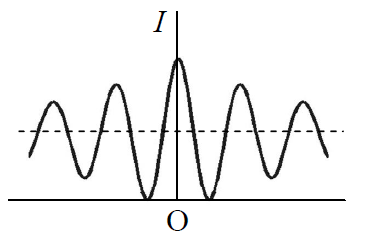
\includegraphics[width=\textwidth]{5b.png}
            \caption*{б)}
        \end{subfigure}
        \caption{}
        \label{fig5:schema}

    \end{figure}

    Через це результуюча інтенсивність у максимумах буде поступово зменшуватись,
    а в мінімумах --- збільшуватись, і смуги в решті решт зникнуть, рис. 5б
    Це станеться тоді, коли максимум якогось порядку $m'$ для довжини
    хвилі $\lambda + \Delta \lambda$ співпаде з мінімумом порядку $m'$ для довжини
    хвилі $\lambda$. Тому з формул (8) і (8а) виходить:

    \begin{center}
        $\displaystyle m' = \frac{\lambda}{2 \Delta \lambda}$.
    \end{center}

    Формально число $m'$ можна трактувати як максимальний порядок інтерференції,
    який можна спостерігати для таких умовних променів. Насправді ж у реальному
    випромінюванні присутня безліч довжин хвиль від $\lambda$ до
    $\lambda + \Delta \lambda$, різниці котрих варіюють в інтервалі
    $0 \div \Delta \lambda$ і в середньому складають $\Delta \lambda / 2$.
    Це покращує умови спостереження, і більш коректно максимальний порядок
    інтерференції виражається числом

    \begin{equation}
        m_{max} = \frac{\lambda}{\Delta \lambda},
        \tag{12}
    \end{equation}

    в якому величина

    \begin{center}
        $\displaystyle \frac{\lambda}{\Delta \lambda} = \frac{\omega}{\Delta \omega}$
    \end{center}

    задає ступінь монохроматичності, тобто наближеності світла до строго монохроматичного.

    Таким чином, неповна монохроматичність світла обмежує кількість інтерференційних смуг,
    які можна спостерігати на екрані, величиною

    \begin{equation}
        N \leq 2m_{max} = 2\frac{\lambda}{\Delta \lambda}.
        \tag{12а}
    \end{equation}

    Із цього виразу в даній роботі, підрахувавши максимальну кількість
    смуг $N \approx 2m_{max}$, які спостерігаються, і попередньо визначену
    довжину хвилі $\lambda$, можна оцінити ширину смуги пропускання світлофільтра $\Delta \lambda$:

    \begin{equation}
        \Delta \lambda \approx \frac{2 \lambda}{N}.
        \tag{13}
    \end{equation}

    В умовах даної роботи можна спостерігати тільки досить обмежену кількість
    смуг $N$ з малою шириною смуги $\Delta x$. Тому смуги спостерігаються лише в
    малій області біля центра екрана шириною $L = N\Delta x$.

    Негативний вплив на інтерференцію спричинюють і лінійні розміри
    джерела світла. Це пояснюється тим, що когерентні промені, які приходять у
    точку спостереження від різних ділянок протяжних джерел, мають не однакові різницю
    ходу та різницю фаз. Тому в інтерференційній формулі (3) значення
    $\langle \cos \delta \rangle$ є усередненим не тільки по часу, а й по всіх елементарних
    ділянках джерел, від яких приходять промені в точку спостереження.
    Як наслідок в усіх точках спостереження величина $\langle \cos \delta \rangle$ виявляється меншою, ніж
    у випадку точкових джерел. Через це зменшується різниця інтенсивностей
    максимумів і мінімумів, тобто погіршується контрастність інтерференційних
    смуг. Так що при великих розмірах джерел смуги взагалі зникають навіть при
    дуже високому ступені монохроматичності випромінювання. Тому в кожному конкретному
    випадку існують певні граничні розміри джерел, при яких ще можна спостерігати
    інтерференцію. Зокрема, у досліді з біпризмою Френеля інтерференційні смуги теоретично
    можна спостерігати лише коли ширина щілини $b$ є меншою за ширину інтерференційної смуги (9):

    \begin{center}
        $\displaystyle b < \frac{\lambda l}{h}$.
    \end{center}

    Таким чином, через неповну монохроматичність і скінченні лінійні
    розміри джерел, на практиці можна спостерігати тільки обмежену кількість
    інтерференційних смуг і лише при малих розмірах та достатньому ступені
    монохроматичності джерел.

    \newpage

    \begin{center}
        \textbf{\Large Практична частина}
    \end{center}

    \begin{center} \textbf{Установка для спостережень і вимірів} \end{center}

    Експериментальна установка являє собою оптичну лаву --- масивну рейку з напрямними
    на якій на спеціальних підставках (рейтерах) установлені всі елементи оптичної схеми
    (рис.6а).

    \begin{figure}[h!]
        \centering
        
        % Підрисунок а)
        \begin{subfigure}[b]{0.8\textwidth}
            \centering
            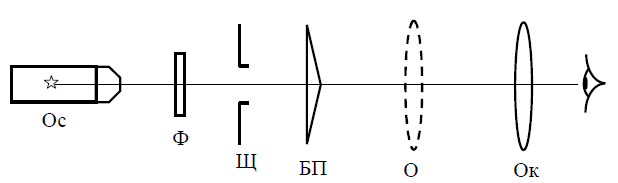
\includegraphics[width=\textwidth]{6a.png} % ← Заміни на своє ім’я файлу
            \caption*{а)}
        \end{subfigure}
        
        \vspace{1em} % відступ між підрисунками
        
        % Підрисунок б)
        \begin{subfigure}[b]{0.8\textwidth}
            \centering
            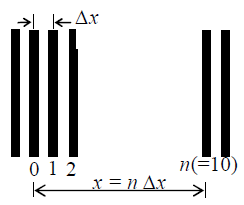
\includegraphics[width=0.4\textwidth]{6b.png} % ← Заміни на своє ім’я файлу
            \caption*{б)}
        \end{subfigure}
        
        \caption{}
        \label{fig:6}

    \end{figure}

    Пучок світла від освітлювача Ос проходить через змінний світлофільтр Ф
    і потрапляє на розсувну щілину Щ, яка виконує роль лінійного джерела, а
    потім на біпризму Френеля БП.

    Інтерференційна картина, що виникає при накладенні когерентних пучків від біпризми,
    спостерігається через окуляр Ок. У полі зору окуляра око
    бачить збільшене зображення інтерференційних смуг які схематично зображені на рис. 6б,
    а також вертикальну візирну нитку та горизонтальну шкалу для визначення координат і
    ширини інтерференційних смуг.
    
    Для визначення відстані між уявними когерентними джерелами, утвореними біпризмою,
    між нею та окуляром установлюється допоміжний об’єктив О --- збірна лінза з відомою
    фокусною відстанню $F$.

    \begin{center} \textit{Налаштування установки.} \end{center}

    Для спостереження чітких інтерференційних смуг і проведення якісних вимірів
    установка має бути відповідно налаштована або, як говорять --- від'юстована.
    Для цього передбачена можливість переміщення всіх елементів як уздовж, так
    і впоперек осі системи. Для налаштування необхідно:

    \begin{itemize}

        \item при ширині щілини $\approx$ 1 мм установити елементи системи так, щоби щілина й
        ребро біпризми були паралельними, а світловий пучок від щілини порівну освітлював
        половинки біпризми і після неї потрапляв до окуляра;

        \item поступово зменшувати ширину щілини до появи в полі зору окуляра світлих і
        темних смуг. Зменшувати ширину щілини далі до величини,
        при якій ще забезпечується необхідна для спостережень яскравість картини;

        \item акуратно повертаючи біпризму на малий кут навколо осі системи,
        підібрати таке положення, при якому інтерференційна картина в окулярі буде
        максимально чіткою;

        \item при всіх наступних діях положення елементів системи має лишатися незмінним.
    
    \end{itemize}

    \begin{center} \textbf{Виміри} \end{center}

    \begin{center} \textit{Визначення координат і кількості інтерференційних смуг} \end{center}

    Для кожного із змінних світлофільтрів:

    \begin{enumerate}
        \item Переміщуючи окуляр за допомогою мікрометричного гвинта, виставити візирну
        лінію на якусь темну смугу з лівого краю інтерференційної картини і приписати
        їй номер 0. Зафіксувати координату цієї смуги $x_0$ по лімбу мікрометра;

        \item Перемістити візирну лінію на якусь темну смугу, наприклад з номером
        $n = 10$, у правій частині інтерференційної картини і зафіксувати її координату $x_n$;

        \item Вирахувати різницю координат $X = x_n - x_0$ і занести її до таблиці №1.
        
        Виміри п.п. 1-3 повторити 3 рази.

        \item Підрахувати загальну кількість смуг $N$, які можна розрізнити в полі
        зору окуляра, та занести її до таблиці №1.

    \end{enumerate}

    \begin{center} \textit{Визначення відстані між уявними джерелами та довжини хвилі} \end{center}

    \begin{enumerate}

        \item Установити на рейці між біпризмою та окуляром допоміжний
        об'єктив О; пересуваючи його по рейці, отримати в полі зору окуляра Ок дві
        яскраві та максимально різкі лінії, що є зображеннями уявних когерентних
        джерел створених біпризмою.

        Хід променів через об’єктив, положення джерел $S_1$ i $S_2$ та їхніх зображень 
        $S_1'$ і $S_2'$, а також потрібні відстані показані на рис. 7;

        \begin{figure}[!ht]

            \renewcommand{\thefigure}{\arabic{figure}} % робимо "3.1", "3.2" і т.д.
    
            \centering
            % Підставляєте потрібний шлях та розмір зображення:
            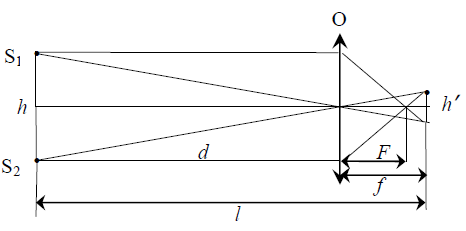
\includegraphics[width=0.5\textwidth]{7.png}
            % Підпис (зазвичай під малюнком):
            \caption{}
            % Мітка для посилань у тексті (\ref{fig:...})
            \label{fig7:schema}
    
        \end{figure}

        \item Виміряти відстань $d$ від щілини до площини об'єктива.
        Занести її та фокусну відстань об'єктива $F$ до таблиці №1.

        \item Для якогось одного світлофільтра за допомогою окуляра виміряти відстань
        $h$ між зображеннями когерентних джерел, як описано в п.1. 
        Вимірювання провести 3 рази і результати занести до таблиці №1.

    \end{enumerate}

    Відстань $h$ між самими джерелами, яка потрібна для визначення за формулою (9)
    довжини хвилі в максимумі пропускання фільтра, знаходиться через величину
    $h'$ за допомогою формули лінзи наступним чином.

    З рис. 7 видно, що

    \begin{equation}
        \frac{h}{h'} = \frac{d}{F} \quad \text{і} \quad f = l - d \quad \Rightarrow \quad h = \frac{d}{l-d}h'.
        \tag{14}
    \end{equation}

    Відтак формулу (9) можна переписати у вигляді:

    \begin{equation}
        \lambda = \frac{\Delta xd}{l(l-d)}h'.
        \tag{15}
    \end{equation}

    Величину $l$, яку не можна виміряти безпосередньо, виражаємо з формули лінзи:

    \begin{equation}
        \frac{1}{d} + \frac{1}{f} = \frac{1}{F} \quad \Rightarrow \quad l = \frac{d^2}{d - F}
        \tag{16}
    \end{equation}

    Після підстановки цього виразу в (15) отримуємо робочу розрахункову формулу для довжини хвилі:

    \begin{equation}
        \lambda = \frac{\Delta xh' \left( d - F \right)^2}{d^2 F}
        \tag{17}
    \end{equation}

    \begin{center} \textit{Додаткове завдання (виконується за вказівкою викладача)} \end{center}

    Прибрати світлофільтр і спостерігати інтерференційну картину в білому
    світлі $\lambda \approx (400 \div 800)$ нм;
    підрахувати та занести до таблиці №1 максимальну кількість смуг $N'$, що спостерігаються.

    \newpage

    \begin{center} \textbf{Порядок виконання} \end{center}

    \begin{enumerate}
        \item \textbf{Підготовка установки:}
        \begin{itemize}
          \item Зібрав експериментальну установку з біпризмою Френеля.
          \item Налаштував положення щілини та біпризми так, щоб світловий пучок рівномірно освітлював обидві половини біпризми.
          \item Зменшував ширину щілини до отримання чіткої інтерференційної картини в окулярі.
        \end{itemize}
      
        \item \textbf{Вимірювання ширини інтерференційної смуги:}
        \begin{itemize}
          \item Встановив візирну лінію на темну смугу №0 (лівий край) та зафіксував координату.
          \item Визначив координату смуги з номером $n = 10$ праворуч.
          \item Провів 3 серії вимірювань для кожного світлофільтра (червоного і зеленого).
          \item Обчислив середнє значення $\langle x_i \rangle$ та ширину смуги $\displaystyle \Delta x = \frac{x}{n}$.
        \end{itemize}
      
        \item \textbf{Визначення відстані між уявними джерелами:}
        \begin{itemize}
          \item Встановив допоміжний об’єктив між біпризмою та окуляром.
          \item За допомогою окуляра провів 3 вимірювання відстані $h'$ між зображеннями уявних джерел та обчислив середнє.
        \end{itemize}
      
        \item \textbf{Розрахунок довжини хвилі та спектральної ширини:}
        \begin{itemize}
          \item Виміряв відстані $d$ і $F$.
          \item Обчислив довжину хвилі $\lambda$ за формулою:
          \[
          \lambda = \frac{\Delta x \cdot h' (d - F)^2}{d^2 F}
          \]
          \item Обчислив ширину смуги пропускання:
          \[
          \Delta \lambda \approx \frac{2\lambda}{N}
          \]
        \end{itemize}
      
        \item \textbf{Оцінка похибок:}
        \begin{itemize}
          \item Обчислив абсолютні та відносні похибки величин: $n$, $N$, $x_i$, $\Delta x$, $h_i'$, $F$, $d$, $\lambda$ та $\Delta \lambda$ за допомогою Python.
        \end{itemize}

        \textbf{Всi вимiрювання проводив у симуляторi лабораторної роботи OP31!}

    \end{enumerate}

    \newpage

    В даній лабораторній роботі, ми фіксуємо (зупиняємось) 10 лінію, тобто $n = 10$.

    \begin{table}[h!]

        \centering
        \begin{tabular}{|c|c|c|}
        \hline
        Світлофільтр & Червоний & Зелений \\
        \hline
        $N$ & 16,00 & 13,00 \\
        \hline
        $x_i$, мм & 2,58 & 1,95\\ \cline{2-3}
        \empty & 2,53 & 2,05\\ \cline{2-3}
        \empty & 2,51 & 2,11\\
        \hline
        $x = \langle x_i \rangle$, мм & 2,54 & 2,04\\
        \hline
        $\Delta x$, мм & 0,254 & 0,204\\
        \hline
        $h_i'$, мм & 0,61 & 0,61\\ \cline{2-3}
        \empty & 0,62 & 0,60\\ \cline{2-3}
        \empty & 0,61 & 0,58\\
        \hline
        $h' = \langle h_i' \rangle$, мм & 0,61 & 0,60\\
        \hline
        $F$, мм & 145,00 & 145,00\\
        \hline
        $d$, мм & 665,57 & 665,57\\
        \hline
        $\lambda$, нм & 656,26 & 516,40\\
        \hline
        $\Delta \lambda$, нм & 82,03 & 79,45\\
        \hline
        \end{tabular}
        \caption{Результати вимірювань для різних світлофільтрів}
        \label{tab:filters}

    \end{table}

    \setlength{\parindent}{0pt}

    Для червоного світлофільтра:

    \vspace{1em}

    $\displaystyle x = \langle x_i \rangle = \frac{2,58 + 2,53 + 2,51}{3} = 2,54$ мм,
    $\displaystyle h'= \langle h_i' \rangle = \frac{0,61 + 0,62 + 0,61}{3} \approx 0,61$ мм.

    $\displaystyle \Delta x = \frac{x}{n} = \frac{2,54}{10} = 0,254$ мм.

    \vspace{1em}

    Обчислимо знаення $\lambda$ (за формулою 17) та $\Delta \lambda$ (за формулою 13) (обчислення проводились за допомогою Python (\hyperlink{listing1}{Лістинг 1.1})):

    \vspace{1em}

    $\displaystyle \lambda = \frac{\Delta xh' \left( d - F \right)^2}{d^2 F} \approx 656,26$ нм, 
    $\displaystyle \Delta \lambda \approx \frac{2 \lambda}{N} \approx 82,03$ нм.

    \vspace{1em}

    Для зеленого світлофільтра:

    \vspace{1em}

    $\displaystyle x = \langle x_i \rangle = \frac{1,95 + 2,05 + 2,11}{3} \approx 2,04$ мм,
    $\displaystyle h'= \langle h_i' \rangle = \frac{0,61 + 0,60 + 0,58}{3} \approx 0,60$ мм.

    $\displaystyle \Delta x = \frac{x}{n} = \frac{2,04}{10} = 0,204$ мм.

    \vspace{1em}

    Обчислимо знаення $\lambda$ (за формулою 17) та $\Delta \lambda$ (за формулою 13) (обчислення проводились за допомогою Python (\hyperlink{listing1}{Лістинг 1.1})):

    \vspace{1em}

    $\displaystyle \lambda = \frac{\Delta xh' \left( d - F \right)^2}{d^2 F} \approx 516,40$ нм,
    $\displaystyle \Delta \lambda \approx \frac{2 \lambda}{N} \approx 79,45$ нм.

    \newpage
    \begin{center} \textbf{Обчислення похибок} \end{center}

    \setlength{\parindent}{1em}

    В даній лабораторні роботі, ми оперували такими величинами: $n$, $N$, $x_i$, $\Delta x$, $h_i'$, $F$, $d$, $\lambda$ та $\Delta \lambda$.
    Тут величини $n$ та $N$ --- цілі числа, які виникли під час лічби, тому їх похибка дорівнює нулю.
    Щодо інших, то розділимо їх на дві групи: величини, які вимірювались безпосередньо (пряме вимірювання) та величини, які обчислювались за формулами (непряме вимірювання).

    Величини прямих вимірювань: $x_i$, $h_i'$, $F$, $d$.
    Величини непрямих вимірювань: $\Delta x$, $\lambda$, $\Delta \lambda$.

    Всі розрахунки похибок виконані за допомогою Python коду (\hyperlink{listing2}{Лістинг 1.2})!

    Почнемо розрахунок похибок із величин прямих вимірювань.

    Для обчислення похибки $x_i$ скорстаємося формулою середньоквадратичної похибки (U-оцінник дисперсії), помноженої на коефіцієнт Стьюдента: з 6 кількістю вимірювань та довірчим коефіцієнтом $\alpha = 0,9$
    коефіцієнт Стьюдента дорівнює $t_{k=6, \alpha = 0,9} = 2,02$. Але так як величину $x_i$ вимірювали при різних світлофільтрах, то я використаю середнє значення абсолютних похибок для окремих світлофільтрів.

    Відносну ж похибку я обчислюватиму як середнє значення відносних похибок для окремих світлофільтрів, які обчислювались як частка абсолютної похибки та значення величини $\langle x_i \rangle$. Тобто

    \begin{center}

        $\displaystyle \delta x_i = \frac{2,02}{2} \cdot \left( \sqrt{\frac{1}{n(n-1)} \sum_{i=1}^n \left( x_{1i} - \langle x_1 \rangle \right)^2 } +
        \sqrt{\frac{1}{n(n-1)} \sum_{i=1}^n \left( x_{2i} - \langle x_2 \rangle \right)^2} \right)$ \\

        $\displaystyle \varepsilon_{x_i} = \frac{1}{2} \left( \frac{\delta x_1}{\langle x_1 \rangle} + \frac{\delta x_2}{\langle x_2 \rangle} \right) \cdot 100\%$

    \end{center}

    За результатами розрахунків програми, $\delta x_i \approx 0,0681$ мм, $\varepsilon_{x_i} \approx 3,14$ \%.

    Щодо величини $h_i'$, то судження тут такі самі. Тобто

    \begin{center}

        $\displaystyle \delta h_i' = \frac{2,02}{2} \cdot \left( \sqrt{\frac{1}{n(n-1)} \sum_{i=1}^n \left( h_{1i}' - \langle h_{1i}' \rangle \right)^2 } +
        \sqrt{\frac{1}{n(n-1)} \sum_{i=1}^n \left( h_{2i}' - \langle h_{2i}' \rangle \right)^2} \right)$ \\

        $\displaystyle \varepsilon_{h_i'} = \frac{1}{2} \left( \frac{\delta h_1'}{\langle h_1' \rangle} + \frac{\delta h_2'}{\langle h_2' \rangle} \right) \cdot 100\%$

    \end{center}

    За результатами розрахунків програми, $\delta h_i' \approx 0,012$ мм,  $\varepsilon_{h_i'} \approx 2,04$ \%.

    Щодо величини $F$, то вона вимірювалась за допомогою лінійки. Тобто задача знаходження абсолютної та відносної похибок $F$
    зводиться до знаходження абсолютної та відносної похибок лінійки. Нехай найменша поділка лінійки дорівнює 1 мм. Тоді абсолютну похибку
    можна обчислити як половину від найменшої поділки лінійки, тобто $\delta F = 0,5$ мм. Відносну ж похибку можна обчислити як частку
    абсолютної похибки та значення величини $F$, тобто $\displaystyle \varepsilon_F = \frac{\delta F}{F} \cdot 100\% = \frac{0,5\cdot 10^{-3}}{145 \cdot 10^{-3}} \approx 0,34 \%$.

    Щодо величини $d$, то судження тут такі самі, як і у $F$. Тобто $\delta d = 0,5$ мм, $\displaystyle \varepsilon_d = \frac{\delta d}{d} = \frac{0,5 \cdot 10^{-3}}{665,57 \cdot 10^{-3}} \approx 0,075 \%$.

    Тепер розглянемо величини непрямих вимірювань.

    Для обчислення похибки $\Delta x$ визначимо, від яких величин вона залежить за її ж формулою:

    \begin{center}
        $\displaystyle \Delta x = \frac{x}{n} = \frac{\langle x_i \rangle}{n}$
    \end{center}

    \newpage

    Тобто $\Delta x$ залежить від величин $\langle x_i \rangle$ та $n$, але оскільки величина $n$ має нульову похибку, то насправді похибка $\Delta x$ прямо залежить від похибки $\langle x_i \rangle$, яку у свою чергу
    ми обчислили раніше, як $\delta x_i$. Тобто $\delta \Delta x = \delta x_i \approx 0,0681$ мм, та $\varepsilon_{\Delta x} = \varepsilon_{x_i} \approx 3,14$ \%.

    Щодо величини $\lambda$, то вона залежить від величин $\Delta x$, $h'$, $d$ та $F$. Тоді абсолютну та відносні похибки я буду обчислювати за Гаусовими формулами обчислення похибок:

    \[
        \delta y \;=\;
        \sqrt{
        \left(
            \frac{\partial f}{\partial a}\Bigg|_{\substack{a=\langle a\rangle \\ b=\langle b\rangle \\ \dots}}
        \right)^{2} S_{(a)}^{2}
        \;+\;
        \left(
            \frac{\partial f}{\partial b}\Bigg|_{\substack{a=\langle a\rangle \\ b=\langle b\rangle \\ \dots}}
        \right)^{2} S_{(b)}^{2}
        \;+\;\dots
        }
    \]

    \[
        \varepsilon_y \;=\;
        \sqrt{
        \left(
            \frac{\partial \ln f}{\partial a}\Bigg|_{\substack{a=\langle a\rangle \\ b=\langle b\rangle \\ \dots}}
        \right)^{2} S_{(a)}^{2}
        \;+\;
        \left(
            \frac{\partial \ln f}{\partial b}\Bigg|_{\substack{a=\langle a\rangle \\ b=\langle b\rangle \\ \dots}}
        \right)^{2} S_{(b)}^{2}
        \;+\;\dots
        } \cdot 100 \%
    \]

    Функція $\lambda$ має такий формульний вигляд:

    \begin{center}
        $\displaystyle \lambda = \frac{\Delta xh' \left( d - F \right)^2}{d^2 F}$
    \end{center}

    Звідси

    \begin{center}
    
        $\displaystyle \frac{\partial \lambda}{\partial \Delta x} = \frac{h' (d - F)^2}{d^2 F}, \quad
        \frac{\partial \lambda}{\partial h'} = \frac{\Delta x (d - F)^2}{d^2 F}, \quad$ \\[0.5em]
        $\displaystyle \frac{\partial \lambda}{\partial d} = 2\frac{\Delta x h' (d - F)}{d^3 F}, \quad
        \frac{\partial \lambda}{\partial F} = -\frac{\Delta x h' \left( d^2 - F^2 \right)}{d^2 F^2}$.

    \end{center}

    \begin{center}
        $\displaystyle \frac{\partial \ln \lambda}{\partial \Delta x} = \frac{1}{\Delta x}, \quad
        \frac{\partial \ln \lambda}{\partial h'} = \frac{1}{h'}, \quad
        \frac{\partial \ln \lambda}{\partial d} = \frac{2}{d - F} - \frac{2}{d}, \quad
        \frac{\partial \ln \lambda}{\partial F} = -\frac{2}{d - F} - \frac{1}{F}.$
    \end{center}

    Звідси формули для розрахунку абсолютної та відносної похибок $\lambda$ будуть:

    \begin{center}
        $\displaystyle \delta \lambda = \left(
            \left(\frac{\langle h' \rangle (d - F)^2}{d^2 F}\,\delta  \Delta x \right)^2 +
            \left(\frac{\langle \Delta x \rangle (d - F)^2}{d^2 F}\,\delta h'\right)^2 +
            \left(2\frac{\langle \Delta x \rangle \langle h' \rangle (d - F)}{d^3 F} \cdot \delta d\right)^2 +
        \right.$ \\
        $\displaystyle \left.
            +\left( \frac{\langle \Delta x \rangle \langle h' \rangle \left( d^2 - F^2 \right)}{d^2 F^2} \cdot \delta F\right)^2 \right)^{1/2}$
    \end{center}

    \begin{center}
        $\displaystyle \varepsilon_\lambda =
        \sqrt{
        \left( \frac{\delta \Delta x}{\langle \Delta x \rangle} \right)^2 +
        \left( \frac{\delta h'}{\langle h' \rangle} \right)^2 +
        \left( \left( \frac{2}{d} - \frac{2}{d - F} \right) \cdot \delta d \right)^2 +
        \left( \left( \frac{1}{F} + \frac{2}{d - F} \right) \cdot \delta F \right)^2
        } \cdot 100 \%$
    \end{center}

    За $\langle \Delta x \rangle$ беремо середнє значення: $\displaystyle \langle \Delta x \rangle = \frac{\Delta x_1 + \Delta x_2}{2} = \frac{0,254 + 0,204}{2} = 0,229$ мм.

    $\displaystyle \langle h' \rangle = \frac{\langle h_1' \rangle + \langle h_2' \rangle}{2} = \frac{0,61 + 0,60}{2} = 0,605$ мм.

    \vspace{1em}

    За результатами виконання програми з \hyperlink{listing2}{Лістингу 1.2}: $\delta \lambda \approx 174,4 \text{нм}, \varepsilon_{\lambda} \approx 29,84$ \%.

    Щодо величини $\Delta \lambda$, то вона має такий формульний вигляд:

    \begin{center}
        $\displaystyle \Delta \lambda \approx \frac{2\lambda}{N}$,
    \end{center}

    тобто вона залежить від 2 змінних: $\lambda$ та $N$, але так як $N$ виникла під час лічби, то вона має нульову похибку, а число 2 --- є константою.
    Це значить, що похибка величини $\Delta \lambda$ прямо залежить тільки від похибки величини $\lambda$, а це значить, що вони співпадають.
    Тобто $\delta \Delta \lambda = \delta \lambda \approx 174,4 \text{нм}, \varepsilon_{\Delta \lambda} = \varepsilon_{\lambda} \approx 29,84$ \%.

    \newpage

    \setlength{\parindent}{0pt}

    \textbf{\underline{Висновок:}}
    \vspace{1em}

    \setlength{\parindent}{1.5em}

    У роботі досліджено інтерференцію світла за допомогою біпризми Френеля. Виміряно ширину інтерференційних смуг та обчислено довжини хвиль:

    \begin{itemize}
        \item $\lambda_{\text{червоного}} \approx 656{,}26\,\text{нм}$;
        \item $\lambda_{\text{зеленого}} \approx 516{,}40\,\text{нм}$.
    \end{itemize}

    Оцінено ширину смуги пропускання світлофільтрів:

    \begin{itemize}
        \item $\Delta \lambda_{\text{червоного}} \approx 82{,}03\,\text{нм}$;
        \item $\Delta \lambda_{\text{зеленого}} \approx 79{,}45\,\text{нм}$.
    \end{itemize}

    Результати узгоджуються з теоретичними розрахунками. Також були обчислені похибки величин:

    \vspace{1em}

    $\delta x_i \approx 0,0681$ мм, $\varepsilon_{x_i} \approx 3,14$ \%,
    
    $\delta h_i' \approx 0,012$ мм, $\varepsilon_{h_i'} \approx 2,04$ \%,

    $\delta F \approx 0,5$ мм, $\varepsilon_F \approx 0,34$ \%,

    $\delta d \approx 0,5$ мм, $\varepsilon_d \approx 0,075$ \%,

    $\delta \Delta x \approx 0,0681$ мм, $\varepsilon_{\Delta x} \approx 3,14$ \%,

    $\delta \lambda \approx 174,4$ мм, $\varepsilon_{\lambda} \approx 29,84$ \%,

    $\delta \Delta \lambda \approx 174,4$ мм, $\varepsilon_{\Delta \lambda} \approx 29,84$ \%.

    \newpage

    \begin{center} \textbf{\large Контрольні питання} \end{center}

    \setlength{\parindent}{0pt}

    \textbf{1. Що називається інтерференцією світла? Виведіть формули (1.1) та (1.2).}

    \setlength{\parindent}{1.5em}

    Інтерференція світла — це явище просторового перерозподілу інтенсивності при накладанні двох або більше когерентних світлових хвиль. \\
    Нехай дві хвилі з електричними полями:
    \[ E_1 = E_{01} \cos(\omega t - k_1 l_1 + \varphi_{01}) = E_{01} \cos(\omega t - \alpha_1), \]
    \[ E_2 = E_{02} \cos(\omega t - k_2 l_2 + \varphi_{02}) = E_{02} \cos(\omega t - \alpha_2). \]
    Різниця фаз:
    \[ \delta = \alpha_1 - \alpha_2 = (k_2 l_2 - k_1 l_1) - \delta_0, \quad \text{де } \delta_0 = \varphi_{02} - \varphi_{01}. \]
    Інтенсивність:
    \[ I = I_1 + I_2 + 2\sqrt{I_1 I_2} \cos \delta. \]
    
    \vspace{1em}
    \setlength{\parindent}{0pt}

    \textbf{2. Які хвилі називаються когерентними? Чому світлові хвилі, що випромінюються незалежними джерелами, некогерентні?}
    \setlength{\parindent}{1.5em}

    Когерентні хвилі — це хвилі з однаковою частотою, сталою різницею фаз і сталим напрямком коливань. Незалежні джерела випромінюють цуги з випадковими фазами, тому різниця фаз між хвилями змінюється з часом, що робить їх некогерентними.

    \vspace{1em}

    \setlength{\parindent}{0pt}

    \textbf{3. Поясніть принцип отримання когерентних світлових хвиль та наведіть приклади.}

    \setlength{\parindent}{1.5em}

    Когерентні хвилі можна отримати поділом світлового пучка від одного джерела на два. Приклади: інтерферометр Юнга, пластинка Ллойда, інтерферометр Маха-Цендера.

    \vspace{1em}

    \setlength{\parindent}{0pt}

    \textbf{4. Чи обов'язково буде інтерференція при накладанні когерентних хвиль:}

    \setlength{\parindent}{1.5em}

    \begin{itemize}
    \item[а)] Звукові хвилі — так, завжди, оскільки вони легко когерентні;
    \item[б)] Світлові хвилі — не завжди; необхідна висока когерентність (монохроматичність, стабільна фаза).
    \end{itemize}

    \vspace{1em}
    \setlength{\parindent}{0pt}

    \textbf{5. Що називається оптичною та геометричною різницею ходу променів?}

    \setlength{\parindent}{1.5em}

    \begin{itemize}
    \item Геометрична різниця ходу: $\Delta l = l_2 - l_1$;
    \item Оптична різниця ходу: $\Delta = n_2 l_2 - n_1 l_1$.
    \end{itemize}

    \vspace{1em}
    \setlength{\parindent}{0pt}

    \textbf{6. Виведіть формулу (1.3). Запишіть $\delta$ через $\lambda'$ у однорідному середовищі.}
    \setlength{\parindent}{1.5em}

    \[ \delta = \frac{2\pi}{\lambda_0} (n_2 l_2 - n_1 l_1) = \frac{2\pi}{\lambda'} \Delta. \]

    \vspace{1em}
    \setlength{\parindent}{0pt}

    \textbf{7. Виведіть умову (1.4).}

    \setlength{\parindent}{1.5em}

    Максимум інтенсивності при $\cos\delta = 1$:

    \[ \delta = 2\pi m \Rightarrow \Delta = m \lambda. \]

    Мінімум при $\cos\delta = -1$:
    \[ \delta = (2m + 1)\pi \Rightarrow \Delta = (2m+1)\frac{\lambda}{2}. \]

    \vspace{1em}

    \setlength{\parindent}{0pt}

    \textbf{8. Виведіть формули (1.5) і (1.6). Чому кути біпризми повинні бути малими?}

    \setlength{\parindent}{1.5em}

    Геометрія інтерференції від лінійних джерел

    \[ \Delta(x) = \frac{h}{l}x. \]

    координати максимумів:

    \[ x_m = m \frac{\lambda l}{h}, \quad \Delta x = \frac{\lambda l}{h}. \]

    Малі кути дозволяють отримати малі $h$, що збільшує ширину смуги $\Delta x$ до помітного розміру.

    \vspace{1em}

    \setlength{\parindent}{0pt}

    \textbf{9. Оцінка максимального кута біпризми.}

    \setlength{\parindent}{1.5em}

    За $\Delta x_0 = 0{,}2$ мм, $a = b = 0{,}5$ м, $\lambda = 600$ нм:
    \[ h = \frac{\lambda(a+b)}{\Delta x_0} = \frac{600 \cdot 10^{-9} \cdot 1}{0{,}2 \cdot 10^{-3}} = 3{,}0 \cdot 10^{-3}\ \text{м}. \]
    \[ \theta = \frac{h}{2a(n - 1)} = \frac{3 \cdot 10^{-3}}{2 \cdot 0{,}5 (1{,}5 - 1)} = 6 \cdot 10^{-3} = 0{,}343^\circ. \]

    \vspace{1em}
    \setlength{\parindent}{0pt}

    \textbf{10. Закон розподілення інтенсивності $I(x)$.}

    \setlength{\parindent}{1.5em}

    \[ I(x) = I_1 + I_2 + 2\sqrt{I_1 I_2} \cos \left(\frac{2\pi}{\lambda} \cdot \frac{hx}{l} \right). \]

    \vspace{1em}
    \setlength{\parindent}{0pt}

    \textbf{11. * Вплив неповної монохроматичності. Вивід (1.7).}

    \setlength{\parindent}{1.5em}

    Смуги зникають, коли максимум однієї довжини хвилі збігається з мінімумом іншої:

    \[ m' = \frac{\lambda}{2\Delta\lambda}, \quad m_{\text{max}} = \frac{\lambda}{\Delta\lambda}. \]
    \vspace{1em}
    \setlength{\parindent}{0pt}

    \textbf{12. Вплив розмірів джерела. Вираз для $b_{\text{max}}$.}
    \setlength{\parindent}{1.5em}

    \[ b < \Delta x = \frac{\lambda l}{h}, \quad \Rightarrow b_{\text{max}} = \frac{\lambda l}{h}. \]

    \newpage

    \setlength{\parindent}{0pt}

    \hypertarget{listing1}{}

    \textbf{\large Лістинг 1.1:}

    \vspace{1em}

    \small{ 

\begin{verbatim}
# Фокусна відстань об'єктива, м
F = 145e-3 

# Відстань від щілини до об'єктива, м
d = 665.57e-3 

# Середнє значення h' для червоного та зеленого світлофільтрів, м
h1 = 0.61e-3  # Червоний світлофільтр
h2 = 0.60e-3  # Зелений світлофільтр

# Кількість інтерференційних смуг для кожного світлофільтра
N1 = 16  # Червоний світлофільтр
N2 = 13  # Зелений світлофільтр

# Ширина інтерференційної смуги для кожного світлофільтра, м
Delta_x1 = 0.255e-3  # Червоний світлофільтр
Delta_x2 = 0.204e-3  # Зелений світлофільтр

# Розрахунок довжини хвилі лямда для кожного світлофільтра за формулою (17)
lambda1 = (Delta_x1 * h1 * (d - F)**2) / (d**2 * F) * 1e9  # Переводимо в нанометри
lambda2 = (Delta_x2 * h2 * (d - F)**2) / (d**2 * F) * 1e9  # Переводимо в нанометри

# Округлення результатів до двох знаків після коми
lambda1 = round(lambda1, 2)
lambda2 = round(lambda2, 2)

# Розрахунок ширини смуги пропускання дельта лямда за формулою (13)
Delta_lambda1 = (2 * lambda1) / N1  # Для червоного світлофільтра
Delta_lambda2 = (2 * lambda2) / N2  # Для зеленого світлофільтра

# Округлення результатів до двох знаків після коми
Delta_lambda1 = round(Delta_lambda1, 2)
Delta_lambda2 = round(Delta_lambda2, 2)

# Виведення результатів для довжини хвиль
print(f"Лямда 1: {lambda1}")  # Довжина хвилі для червоного світлофільтра
print(f"Лямда 2: {lambda2}")  # Довжина хвилі для зеленого світлофільтра

# Виведення результатів для довжини хвиль
print(f"Лямда 1, нм: {lambda1}")  # Довжина хвилі для червоного
світлофільтра
print(f"Лямда 2, нм: {lambda2}")  # Довжина хвилі для зеленого
світлофільтра

# Виведення результатів для ширини смуги пропускання
print(f"Дельта лямда 1, нм: {Delta_lambda1}")  # Ширина смуги
пропускання для червоного світлофільтра
print(f"Дельта лямда 2, нм: {Delta_lambda2}")  # Ширина смуги
пропускання для зеленого світлофільтра
\end{verbatim}
}

    \newpage

    Результат виконання програми з Лістингу 1.1:
    \begin{figure}[ht]
        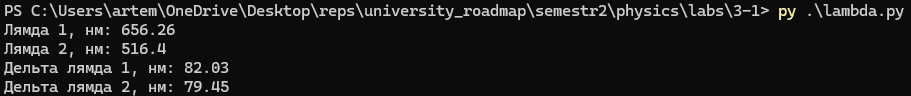
\includegraphics[width=1.0\textwidth]{listing1.png}
    \end{figure}

    \vspace{3em}

    \hypertarget{listing2}{}

    \textbf{\large Лістинг 1.2:}

    \vspace{1em}

    \small{ 

\begin{verbatim}
import numpy as np
import math

# Коефіцієнт Стьюдента для 6 вимірювань і довірчого рівня 90%
STUDENT_COEF = 2.02

# Таблиця виміряних значень x_i для червоного і зеленого
світлофільтрів (у метрах)
X_table = np.array([
    [2.58e-3, 1.95e-3],  # Перше вимірювання
    [2.53e-3, 2.05e-3],  # Друге вимірювання
    [2.51e-3, 2.11e-3]   # Третє вимірювання
])

# Таблиця виміряних значень h_i' для червоного і зеленого
світлофільтрів (у метрах)
h_table = np.array([
    [0.61e-3, 0.61e-3],  # Перше вимірювання
    [0.62e-3, 0.60e-3],  # Друге вимірювання
    [0.61e-3, 0.58e-3]   # Третє вимірювання
])

# ============= X =============

# Абсолютна похибка x_i для кожного світлофільтра
delta_X_vector = np.sqrt(np.var(X_table, ddof=1, axis=0) /
X_table.shape[0]) * STUDENT_COEF
delta_X = np.mean(delta_X_vector)  # Середнє значення абсолютної
похибки
print(f"Абсолютна похибка x_i, мм: {delta_X * 1e3:.3f}")

# Відносна похибка x_i для кожного світлофільтра
relivate1_X = delta_X_vector[0] / np.mean(X_table[:, 0]) * 100 
# Для червоного світлофільтра
relivate2_X = delta_X_vector[1] / np.mean(X_table[:, 1]) * 100 
# Для зеленого світлофільтра

# Середнє значення відносної похибки x_i
relivate_X = (relivate1_X + relivate2_X) / 2
print(f"Відносна похибка x_i, %: {relivate_X:.3f}")

# ============= h' =============

# Абсолютна похибка h_i' для кожного світлофільтра
delta_h_vector = np.sqrt(np.var(h_table, ddof=1, axis=0) /
h_table.shape[0]) * STUDENT_COEF
delta_h = np.mean(delta_h_vector)  # Середнє значення абсолютної похибки
print(f"\nАбсолютна похибка h, мм: {delta_h * 1e3:.3f}")

# Відносна похибка h_i' для кожного світлофільтра
relivate1_h = delta_h_vector[0] / np.mean(h_table[:, 0]) * 100 
# Для червоного світлофільтра
relivate2_h = delta_h_vector[1] / np.mean(h_table[:, 1]) * 100 
# Для зеленого світлофільтра

# Середнє значення відносної похибки h_i'
relivate_h = (relivate1_h + relivate2_h) / 2
print(f"Відносна похибка h: {relivate_h:.3f}")

# ============= lambda =============

# Середнє значення ширини інтерференційної смуги (Delta x)
mean_Delta_x = 0.229e-3  # У метрах
delta_d = delta_F = 0.5e-3  # Абсолютна похибка вимірювань d і
F (у метрах)
mean_h = 0.605e-3  # Середнє значення h' (у метрах)
delta_Delta_x = delta_X  # Абсолютна похибка Delta x

# Виміряні значення F і d (у метрах)
F = 145.0e-3
d = 665.57e-3

# Абсолютна похибка довжини хвилі lambda (за формулою для похибок)
delta_lambda = math.sqrt(
    (mean_h * (d - F)**2 * delta_Delta_x / (d**2 * F))**2 +  #
    Вклад похибки Delta x
    (mean_Delta_x * (d - F)**2 * delta_h / (d**2 * F))**2 +  #
    Вклад похибки h'
    (2 * mean_Delta_x * mean_h * (d - F) * delta_d / d**3)**2 +  #
    Вклад похибки d
    (mean_Delta_x * mean_h * (d**2 - F**2) * delta_F / (d**2 * F**2))**2 
    # Вклад похибки F
)
delta_lambda = round(delta_lambda * 1e9, 2)  # Переводимо в нанометри
та округлюємо

# Відносна похибка довжини хвилі lambda (за формулою для відносних похибок)
relivate_lambda = math.sqrt(
    (delta_Delta_x / mean_Delta_x)**2 +  # Вклад відносної похибки Delta x
    (delta_h / mean_h)**2 +  # Вклад відносної похибки h'
    ((2 / d - 2 / (d - F)) * delta_d)**2 +  # Вклад відносної похибки d
    ((1 / F + 2 / (d - F)) * delta_F)**2  # Вклад відносної похибки F
) * 100
relivate_lambda = round(relivate_lambda, 2)  # Округлюємо до двох
знаків після коми

# Виведення результатів для похибок lambda
print(f"\nАбсолютна похибка lambda, нм: {delta_lambda}")
print(f"Відносна похибка lambda, %: {relivate_lambda}")
\end{verbatim}
}

Результат виконання програми з Лістингу 1.2:
\begin{figure}[ht]
    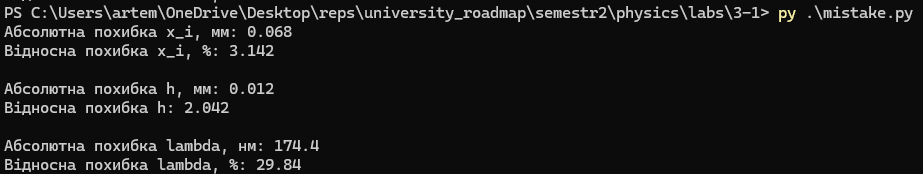
\includegraphics[width=1.0\textwidth]{listing2.png}
\end{figure}


\end{document}